\documentclass[aspectratio=1610]{beamer}
\usepackage[utf8]{inputenc}
\usepackage{polski}
\usepackage[T1]{fontenc}
\usepackage{tikz}
\usepackage{tikzducks}
% \usetikzlibrary{decorations.pathmorphing}
\usepackage{multimedia}
\usepackage{graphicx}
\usepackage[
  % justification=centering, 
  font=scriptsize
]{caption}
\captionsetup[figure]{textfont={small}}
\setbeamerfont{caption}{size=\small}
\usepackage{textcomp}
\usepackage{appendixnumberbeamer}
\usepackage{qrcode}
% \usepackage[natbib, language=polish, sorting=none]{biblatex}
% \addbibresource{lio.bib}
\usepackage{hyperref}
%\usepackage[width=\textwidth]{animate}
%\usepackage{chemformula}
\usepackage{sidecap}
\usepackage{multirow}
\usepackage{multicol}
\usepackage{rotating}
\usepackage{anyfontsize} % change font size for semposiwko

% \usepackage{physics}
\usepackage{array}
\usepackage{booktabs}
\usepackage{transparent}
\usepackage{siunitx}
% \usepackage[rightcaption]{sidecap}
\usepackage{eso-pic}

\usepackage{listings}
\lstset{
basicstyle=\small\ttfamily,
columns=flexible,
breaklines=true
}

% \usepackage{emoji}
\usepackage{subcaption}


\usepackage[natbib, sorting=none]{biblatex}
\addbibresource{lio.bib}
\renewcommand*{\bibfont}{\scriptsize}

\usefonttheme[onlymath]{serif}

\usetheme{Szeged}
\usecolortheme{whale}
\setbeamercolor{palette primary}{bg=violet!80!black,fg=white}
\setbeamercolor{palette secondary}{bg=violet!60!black,fg=white}
% \definecolor{deepviolet}{RGB}{46,0,79}
% \definecolor{vividpink}{RGB}{255,0,127}
% \setbeamercolor{palette primary}{bg=deepviolet,fg=white}
% \setbeamercolor{palette secondary}{bg=vividpink,fg=white}
\setbeamercolor{palette tertiary}{bg=violet!40!black,fg=white}
\setbeamercolor{palette quaternary}{bg=violet!20!black,fg=white}
\setbeamercolor{structure}{fg=violet!60!black}
% \setbeamertemplate{caption}{\insertcaption}
% \setbeamertemplate{headline}{
%   \begin{beamercolorbox}[wd=.9\paperwidth]{headline}
%     \vspace{1.5ex}
%     \insertsectionnavigationhorizontal
%     \vspace{1.5ex}
%   \end{beamercolorbox}
% }
% \definecolor{violet-dark}{HTML}{4B0082}
% \definecolor{teal}{HTML}{008080}
% \definecolor{amber}{HTML}{FFC107}
% \definecolor{light-grey}{HTML}{F5F5F5}
% \definecolor{charcoal}{HTML}{333333}
% \setbeamercolor{palette primary}{bg=violet-dark, fg=white}
% \setbeamercolor{palette secondary}{bg=teal, fg=white}
% \setbeamercolor{palette tertiary}{bg=amber, fg=charcoal}
% \setbeamercolor{background canvas}{bg=light-grey}
% \setbeamercolor{normal text}{fg=charcoal}
% Główna paleta fioletów
% \definecolor{coolblack}{HTML}{000000}
% \definecolor{coolnavy}{HTML}{14213D}
% \definecolor{coolorange}{HTML}{FCA311}
% \definecolor{coollightgray}{HTML}{E5E5E5}
% \definecolor{coolwhite}{HTML}{FFFFFF}

% % Opcjonalnie: ustawienia kolorów dla Beamera
% \setbeamercolor{normal text}{fg=coolblack,bg=coolwhite}
% \setbeamercolor{structure}{fg=coolorange}
% \setbeamercolor{frametitle}{fg=coolwhite,bg=coolnavy}
% \setbeamercolor{title}{fg=coolwhite,bg=coolnavy}
% \setbeamercolor{item}{fg=coolorange}
% \setbeamercolor{block title}{fg=coolwhite,bg=coolnavy}
% \setbeamercolor{block body}{fg=coolblack,bg=coollightgray}
% \setbeamercolor{palette tertiary}{fg=coolwhite, bg=coolorange}
% \setbeamercolor{palette quaternary}{fg=coolblack, bg=coollightgray}

\linespread{0.8}

\setbeamertemplate{background}%
{%
    \begin{tikzpicture}[remember picture,overlay]{\node[yshift=1.5cm,xshift=-2cm,opacity=0.1] at (current page.south east)
      {
      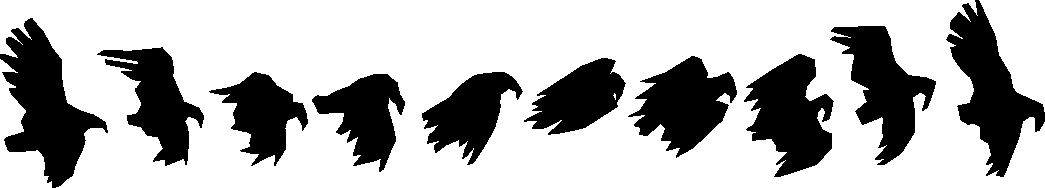
\includegraphics[scale=0.4, angle=25]{ptaki.pdf}
      }
      ;
    \node[yshift=-2cm,xshift=-2cm,opacity=0.1] at (current page.north east)
      {
      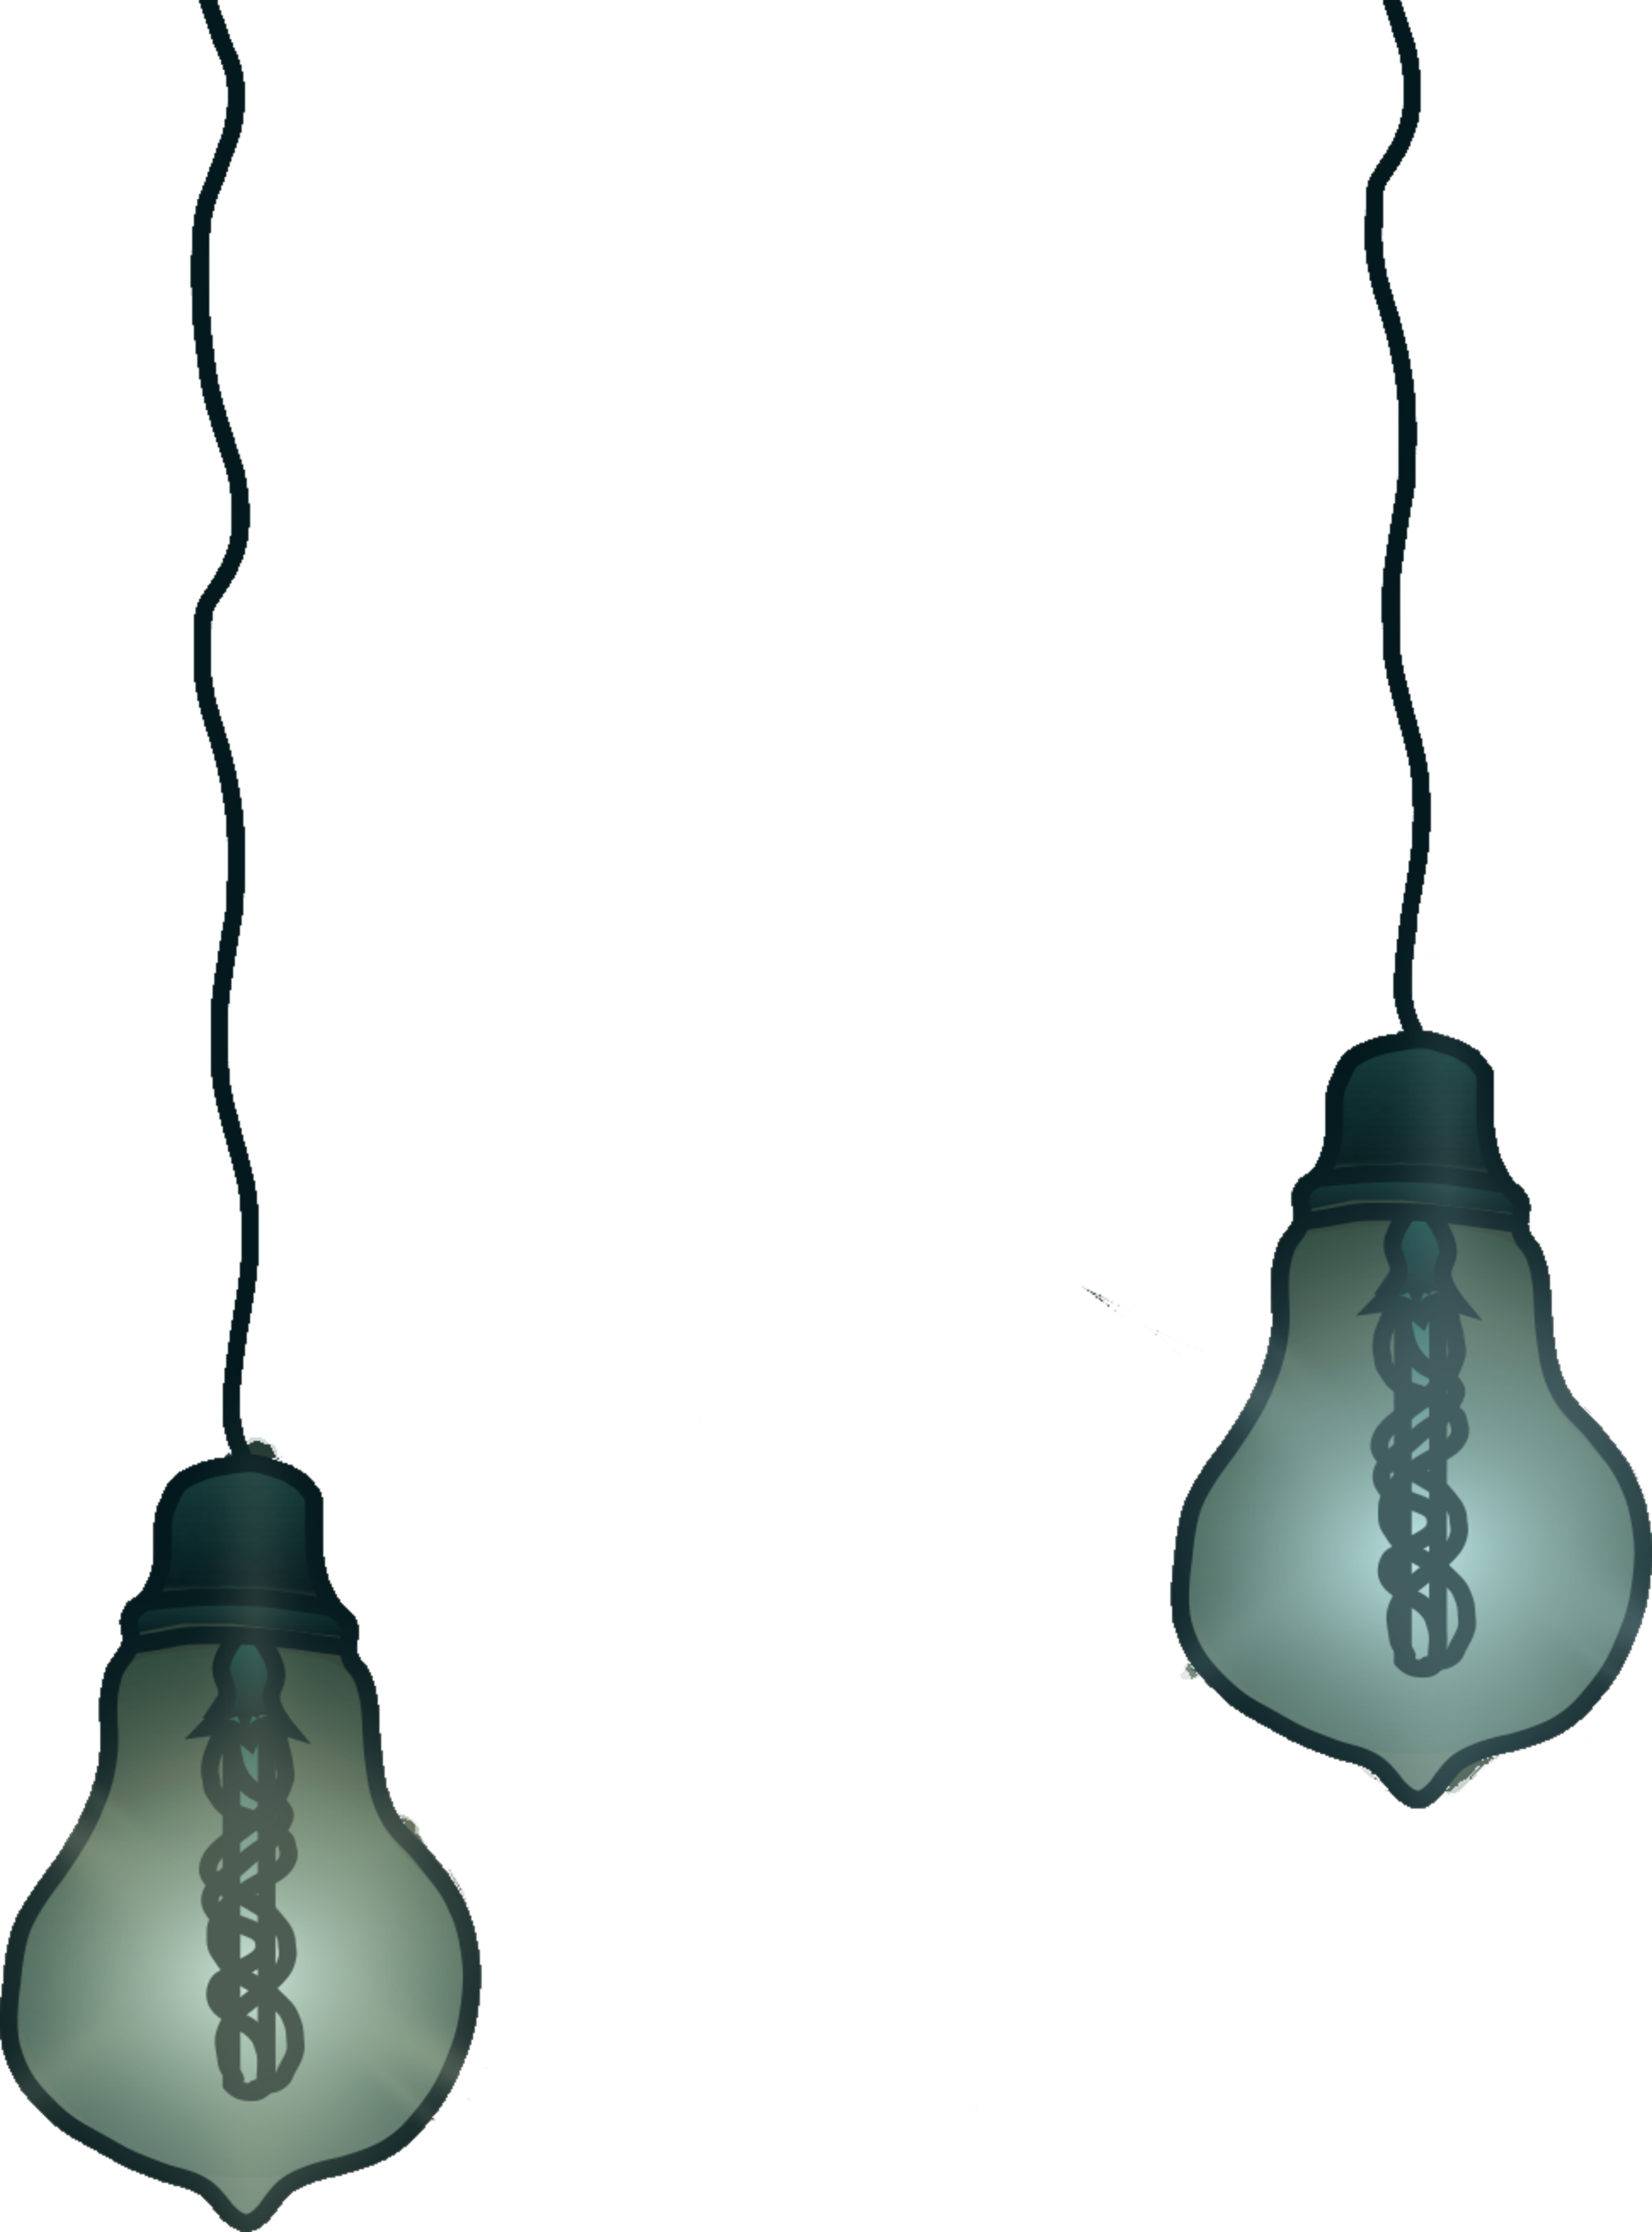
\includegraphics[scale=0.1, angle=0]{zarowki.pdf}
      }
      ;
    \node[yshift=1.0cm,xshift=0.6cm] (logopos) at (current page.south west) {{\begin{tikzpicture}\shuffleducks\duck[signpost=\insertframenumber, \randomhead,scale=.4]\end{tikzpicture}}};
    \pgfmathsetmacro{\progress}{360*(\insertframenumber)/(\inserttotalframenumber)};
    \draw[line width=0.2*3pt] ([xshift=0.55cm] logopos)  arc[radius=0.55cm, start angle=0, end angle=\progress];
    \fill ([shift={(\progress:0.55cm)}] logopos) circle(1pt);

    }
        \end{tikzpicture}
    
}

\newcommand{\SeMPowisko}{%
\large S\normalsize%
\kern-.3em \lower.2ex\hbox{e}%
\lower.2ex\hbox{\large M\normalsize}%
\kern-.1em \raise.1ex\hbox{\large P\normalsize}%
\kern-.3em \lower.2ex\hbox{o}%
\kern-.2em \raise.2ex\hbox{w}%
\lower.2ex\hbox{i}%
s%
\raise.2ex\hbox{k}%
\kern-.3em \lower.2ex\hbox{o}%
}
% \usepackage{microtype}
% \DeclareRobustCommand{\SeMPowisko}{SeMPowisko}


% \newcommand\Tikz{Ti\emph{k}Z}
% \definecolor{neworange}{RGB}{255,140,0}
% \renewcommand{\figurename}{figure}


\title{Elektromagnetycznie indukowana przezroczystość}
% \subtitle{Building a Low-Cost Ground Station with SatNOGS}
\author[M. Winiarski]{Mateusz ,,\(\blacksquare\)'' Winiarski}
\institute[Fizyka atomowa]{fizyka\(^\dagger\), FAIS, Uniwersytet Jagielloński} 
\date[dzisiaj]{dzisiaj, \today}

\begin{document}

\frame{\titlepage}

\section{Teoria}

\begin{frame}{Zjawisko}
\begin{figure}
  \begin{columns}
  \column{0.4\textwidth}
 \centering
 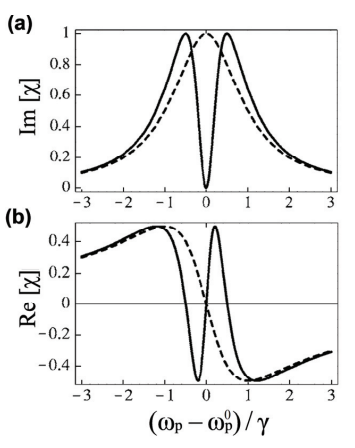
\includegraphics[width=\textwidth]{images/2025-06-05-22-39-37.png}
 \column{0.5\textwidth}
\caption{
Profile podatności elektromagnetycznej \(\chi(\omega_p)\) nieruchomego gazu atomowego w pobliżu rezonansu atomowego \(\omega_p = \omega_p^0\).
\newline
(a) Część urojona podatności \(\mathrm{Im}[\chi(\omega_p)]\) proporcjonalna do współczynnika absorpcji (zgodnie ze wzorem (1));
\newline
(b) Część rzeczywista \(\mathrm{Re}[\chi(\omega_p)]\) związana ze współczynnikiem załamania (zgodnie ze wzorem (2)).
\newline
 Linia przerywana: profil bez wiązki sprzęgającej.
\newline
 Linia ciągła: profil w obecności silnej rezonansowej wiązki sprzęgającej generującej EIT.
\newline
Parametr \(\gamma\): radiacyjna szerokość rezonansu sondy przy braku sprzężenia. (za: \cite{Kowalski_2010})
}
  
\end{columns}
 \end{figure}
\end{frame}

\begin{frame}{Konfiguracje}
\begin{figure}
 \centering
 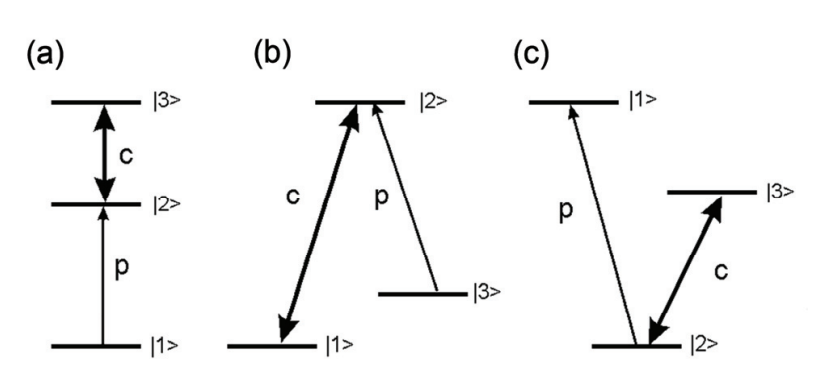
\includegraphics[width=0.9\textwidth]{images/2025-06-05-22-17-00.png}
 \caption{Najprostsze konfiguracje EIT: a) kaskadowa (drabinowa), b) $\Lambda$, c) $V$. Oznaczono: $p$~--~laser próbkujący, $c$ -- silne sprzężenie (za: \cite{Kowalski_2010})}
 \end{figure}
\end{frame}

\begin{frame}{Generacja EIT}
  \begin{figure}
 \centering
 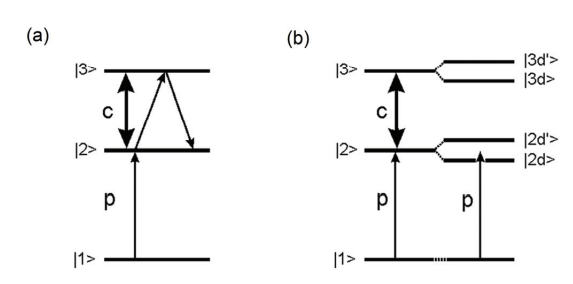
\includegraphics[width=0.7\textwidth]{images/2025-06-05-23-05-26.png}
\caption{%
Schematy dwóch obrazów (mechanizmów) generowania EIT, jako przykład użyto konfiguracji kaskadowej. 
Zmniejszenie absorpcji wynika z destruktywnej interferencji amplitud dla dwóch ścieżek prowadzących do wzbudzenia stanu \(|2\rangle\).
\newline
(a) Przejścia między stanami gołymi (bare states): \(|1\rangle \rightarrow |2\rangle\) oraz \(|1\rangle \rightarrow |2\rangle \rightarrow |3\rangle \rightarrow |2\rangle\);
\newline
(b) Przejścia do bliskich stanów ubranych (dressed-atom states): \(|1\rangle \rightarrow |2_d\rangle\) oraz \(|1\rangle \rightarrow |2_d'\rangle\). 
(za: \cite{Kowalski_2010})%
}

% \newline
% (Szczegółowe wyjaśnienia w tekście)
% } 
\end{figure}
\end{frame}

\section{Eksperyment}

\begin{frame}{Eksperyment: Sr}

  \begin{figure}
 \centering
\begin{columns}
\column{0.5\textwidth}
\centering
 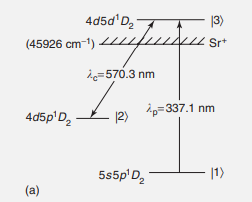
\includegraphics[width=0.7\textwidth]{images/2025-06-05-23-36-41.png}\small
 \caption{\small Elektromagnetycznie indukowana przezroczystość w parach Sr (5s) (a) Poziomy energetyczne Sr i konfiguracja $\Lambda$ ze sprzęgającą i sondującą wiązką o długościach fali $\lambda_c$ i $\lambda_p$, odpowiednio. Transmisja w funkcji odstrojenia lasera sondującego poza rezonans przy braku (b) lub w obecności (c) wiązki sprzęgającej. W warunkach tego eksperymentu pozycja przezroczystości zmienia się z zera do $\sim$40\%. (za: \cite{Harris_1997,Artoni_2005})}
\column{0.5\textwidth}
\centering
% \vspace{5.5cm}
 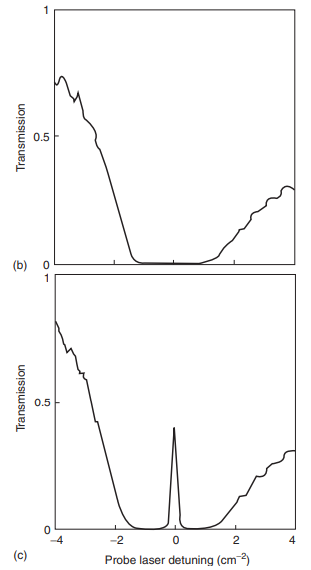
\includegraphics[width=0.6\textwidth]{images/2025-06-05-23-36-13.png}

 ~
\end{columns}
 \end{figure}

\end{frame}

\begin{frame}{Eksperyment: Rb}
  \begin{columns}
  \column{0.4\textwidth}
\begin{figure}
 \centering
 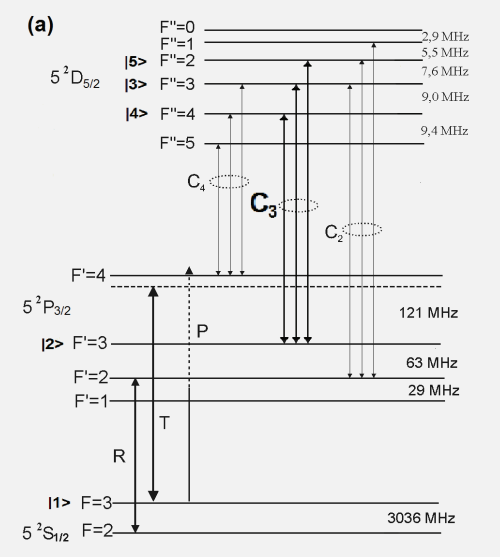
\includegraphics[width=0.9\textwidth]{images/2025-06-06-09-01-02.png}
 \caption{Schemat poziomów energetycznych w atomach $^{85}$Rb }
 \end{figure}

  \column{0.6\textwidth}
\begin{figure}
 \centering
 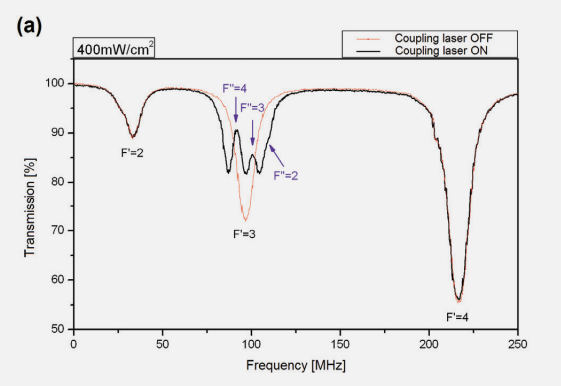
\includegraphics[width=0.8\textwidth]{images/2025-06-06-09-07-34.png}
 \caption{{\scriptsize Przykład spektrum transmisyjnego sondy zarejestrowanych w eksperymentach EIT dla zimnych atomów $^{85}$Rb w MOT. Sonda jest strojona przez przejścia $5S_{1/2}(F = 3) \rightarrow 5P_{1/2}(F' = 2, 3, 4)$. Poziom $5P_{1/2}(F' = 3)$ jest sprzężony do trzech poziomów $5D_{5/2}(F'' = 4, 3, 2)$. Częstotliwość lasera sprzęgającego jest ustawiona blisko środka przejścia $C_a$ (a). (za: \cite{Kowalski_2010})}}
 \end{figure}

  \end{columns}
\end{frame}


\section{Ograniczenia}

\begin{frame}{Czy możemy świecić laserem przez ścianę?}
  \pause
  Nie\pause, ponieważ:
  \begin{itemize}
    \item liczba fotonów w impulsie lasera sprzęgającego $>$ liczba atomów w medium $\times$ siła oscylatora przejścia
    \item moc lasera musi być na tyle duża, by szerokość okna transmisyjnego EIT przekroczyła szerokość linii rezonansu Ramana w materiale
    \item długość impulsów laserowych $<$ czas dekoherencji ($\tau_{deph}$) przejścia Ramana
    \item EIT działa optymalnie dla prostych układów (trójpoziomowych)
  \end{itemize}

\end{frame}

\begin{frame}{}
\begin{figure}
  \begin{columns}
  \column{0.5\textwidth}
 \centering
 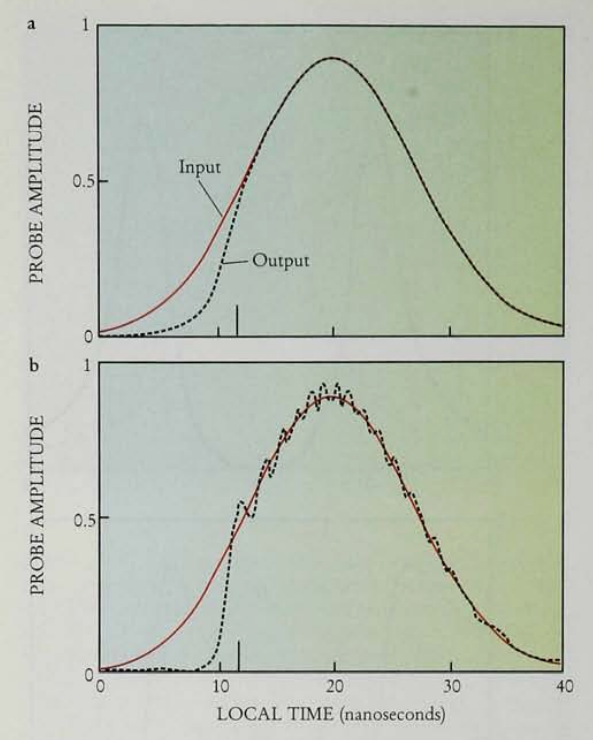
\includegraphics[width=0.8\textwidth]{images/2025-06-06-00-48-29.png}
  \column{0.5\textwidth}
 \caption{Jeśli zastosuje się dopasowane impulsy do optycznie gęstego ośrodka, impulsy samoistnie ustanowią stan uwięziony populacyjnie, i przez cały czas będą następnie transmitowane bez dalszych strat. Oba wykresy pokazują impuls na wejściu (linia ciągła) i na wyjściu (linia przerywana) ośrodka. W obu częściach iloczyn gęstości atomów i długości jest taki sam. Ale w a, strata dla sondy jeśli sama wynosi exp(-5), podczas gdy w b, strata dla sondy jeśli sama wynosi exp(-5000). Duży znacznik w każdym wykresie oznacza czas, w którym wymóg energetyczny jest spełniony. Z grubsza, we wcześniejszych czasach ośrodek jest przygotowywany, a w późniejszych czasach jest przezroczysty. (za: \cite{Harris_1997})}
  \end{columns}
 \end{figure}
\end{frame}


\section{Zatrzymywanie światła}

\begin{frame}{Zatrzymywanie światła: eksperyment z 2013 roku}
  % \begin{itemize}
  %   \item \textbf{Zatrzymywanie światła} to zjawisko, w którym światło jest spowolnione lub zatrzymane w medium.
  %   \item Wykorzystuje się do tego zjawisko \textbf{elektromagnetycznie indukowanej przezroczystości (EIT)}.
  %   \item EIT polega na zmianie absorpcji medium pod wpływem pola elektromagnetycznego.
  % \end{itemize}

\begin{figure}
 \centering
 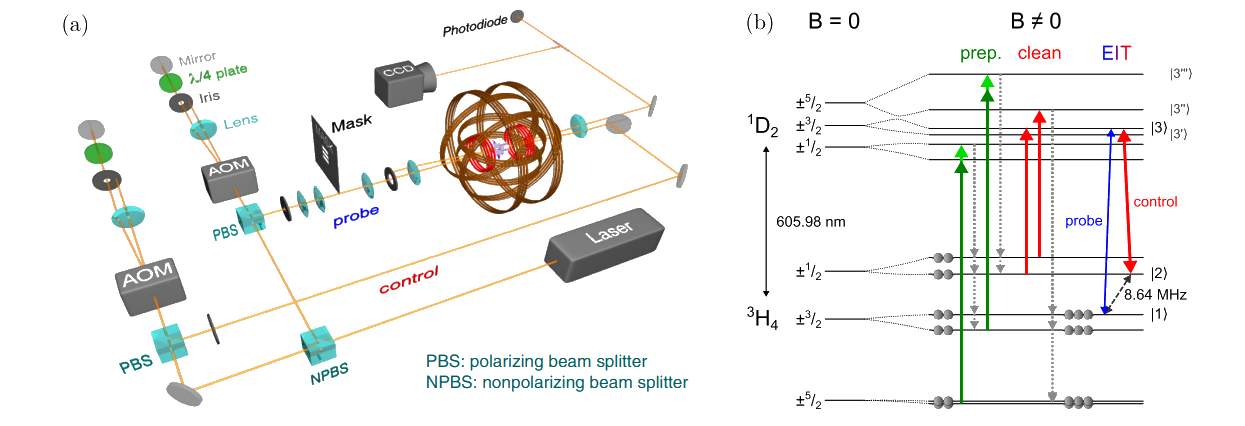
\includegraphics[width=0.95\textwidth]{images/2025-06-05-15-46-32.png}
 \caption{(a) Układ eksperymentalny. (b) Diagram poziomów energetycznych pojedynczego zespołu jonów Pr$^{3+}$, bez i z zewnętrznym polem magnetycznym. Zielone strzałki wskazują działanie drugiego etapu sekwencji impulsów przygotowawczych na rozkład populacji w określonym zespole. Szare, przerywane strzałki wskazują procesy rozpadu podczas pompowania optycznego. Czerwone strzałki wskazują dodatkowy impuls czyszczący. (za: \cite{Heinze_Hubrich_Halfmann_2013})}
 \end{figure}
  
\end{frame}

\begin{frame}{Zatrzymywanie światła: eksperyment z 2013 roku}
  \begin{figure}
 \centering
 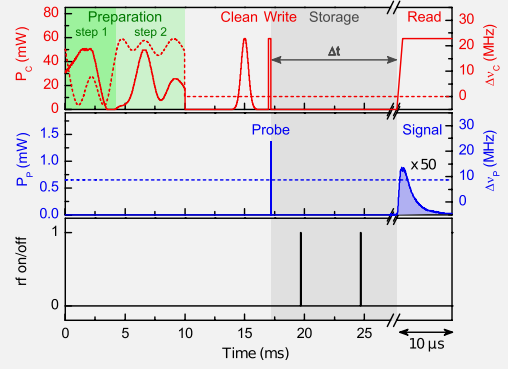
\includegraphics[width=0.5\textwidth]{images/2025-06-05-16-31-24.png}
 \caption{{\scriptsize Sekwencja impulsów sterujących, sondujących i częstotliwości radiowej (rf) w eksperymencie. Trzy wykresy pokazują profile mocy i częstotliwości optycznego impulsu sterującego ($C$), optycznego impulsu sondującego ($P$), i impulsów rf przekształcających. Profile mocy (oś lewa) są rysowane jako linie ciągłe, a częstotliwości (oś prawa) jako linie przerywane. Definiujemy wszystkie częstotliwości jako odstrojenia względem przejścia sterującego. Dla lepszej widoczności przerwano i rozciągnięto oś czasu podczas końcowego etapu odzyskiwania. (za: \cite{Heinze_Hubrich_Halfmann_2013})}}
 \end{figure}
\end{frame}

\begin{frame}{Zatrzymywanie światła: eksperyment z 2013 roku}
\begin{figure}
 \centering
 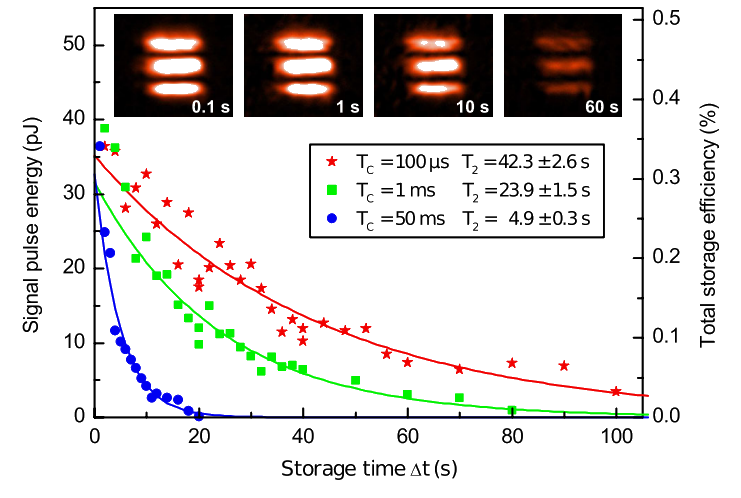
\includegraphics[width=0.5\textwidth]{images/2025-06-05-16-11-39.png}
 \caption{{\scriptsize Energia impulsu sygnałowego i odzyskane obrazy w funkcji czasu przechowywania. Trzy zestawy danych odpowiadają różnym czasom cyklowania w sekwencji dynamicznego sprzęgania: $T_C$ = 100 \si{\micro\second}, $T_C$ = 1 ms, i $T_C$ = 50 ms. Dane są dopasowane przez rozpady eksponencjalne. Dynamiczne sprzęganie przy najszybszym czasie cyklowania skutkuje czasem przechowywania $T_2$ = 42,3 s (czas $1/e$). Wstawki pokazują wyniki przechowywania i odzyskiwania obrazów w układzie, z czasami przechowywania $\Delta t$ wynoszącymi 0,1, 1, 10, i 60 s (od lewej do prawej). Do przechowywania obrazów użyto sekwencji sprzęgania z czasem cyklowania $T_C$ = 100 \si{\micro\second}. (za: \cite{Heinze_Hubrich_Halfmann_2013})}}
 \end{figure}
\end{frame}

\section{~}

\begin{frame}{Bibliografia}{}
  \nocite{*}
  \printbibliography[heading=none]
\end{frame}


\begin{frame}{~}{}
  \transglitter
  \vspace{-1cm}
\begin{figure}
\centering
  \begin{tikzpicture}
    \duck[parrot, body=gray!30!yellow, head=gray!30!yellow, bill=red, torch=gray!70!brown, tshirt=blue!40!black, ribbon=gray, bowtie=blue!50!white, crazyhair=black]
    %\addwater{blue!50!cyan}
    \fill[cyan!20!white] (-1.4,1.8) ellipse (1.8 and 0.5);
\fill[cyan!20!white] (-0.2,1.54) -- (0.2,1.35) -- (0.0,1.6) -- cycle;
\node at (-1.4,1.8) {dziękuję za uwagę};
  \end{tikzpicture}
  \end{figure}


  
  \begin{figure}
  \centering
        % 
\includegraphics[height=0.3\linewidth]{images/2025-05-13-15-25-41.png}\\
      \qrcode[height=0.3\textwidth]{https://github.com/falcotinnunculus/przezrocza/blob/wladca/el-przezrocza/przezrocza.pdf}
  {\scriptsize \url{https://github.com/falcotinnunculus/przezrocza/blob/wladca/el-przezrocza/przezrocza.pdf}}

  \end{figure}
% \vspace{-5.3cm}
% \transparent{0.7}
  % \begin{figure}
      % \centering
      % \caption{Caption}
      % \label{fig:enter-label}
  % \end{figure}
\end{frame}

\end{document}